\documentclass[../main.tex]{subfiles}
\graphicspath{{\subfix{../images/}}}
\begin{document}

\subsection{Dataset}

A collection of 4500 image of each category of fruit were collected from various sources including the internet to help train this model. To avoid data leakage during testing, 300 images from each category were removed to become the testing set and 200 images were removed to become the validation set. 

There is a lot of variations within the set of images. The quantity of the fruit present in the image varies from image to image, some contains only 1 fruit whereas some contains many. While commonly cherries, strawberries, and tomatoes are red, there are also have different colours which indicates its type or ripeness. We also notice that each fruit is a different type of red with cherries having a darker red, strawberries having a vibrant red and tomatoes having a lighter red. Images of the fruits sliced are also included and it contains distinctive patterns on the inside.  

\begin{figure}[h!]
  \centering
  \begin{subfigure}[b]{0.2\linewidth}
    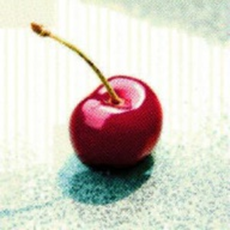
\includegraphics[width=\linewidth]{01-img-variations/single-cherries.png}
  \end{subfigure}
  \begin{subfigure}[b]{0.2\linewidth}
    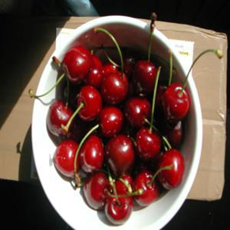
\includegraphics[width=\linewidth]{01-img-variations/multiple-cherries.png}
  \end{subfigure}
  \begin{subfigure}[b]{0.2\linewidth}
    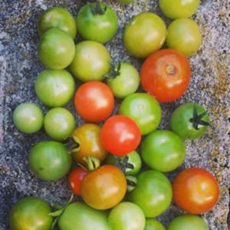
\includegraphics[width=\linewidth]{01-img-variations/colored-tomatoes.png}
  \end{subfigure}
  \begin{subfigure}[b]{0.2\linewidth}
    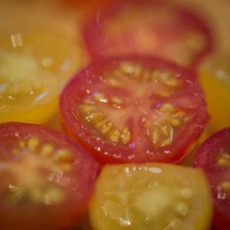
\includegraphics[width=\linewidth]{01-img-variations/sliced-tomatoes.png}
  \end{subfigure}
  \caption{Variations of fruit}
  \label{fig:img-variations}
\end{figure}

Amongst the images there are also images that are not the fruit being classified. We also see that paintings and clip art are also included which are not good representation of the fruit. As we want to classify images of real fruit, these images should not be included in our dataset. 

\begin{figure}[h!]
  \centering
  \begin{subfigure}[b]{0.2\linewidth}
    
\includegraphics[width=\linewidth]{02-invalid-fruits/motel.png}
  \end{subfigure}
  \begin{subfigure}[b]{0.2\linewidth}
    
\includegraphics[width=\linewidth]{02-invalid-fruits/ketchup.png}
  \end{subfigure}
  \begin{subfigure}[b]{0.2\linewidth}
    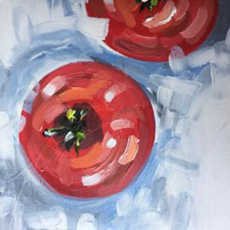
\includegraphics[width=\linewidth]{02-invalid-fruits/painting.png}
  \end{subfigure}
  \begin{subfigure}[b]{0.2\linewidth}
    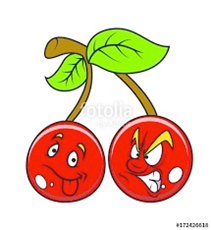
\includegraphics[width=\linewidth]{02-invalid-fruits/cartoon.png}
  \end{subfigure}
  \caption{Invalid Images}
  \label{fig:img-invalid}
\end{figure}

There are also various quality differences within our data. Some fruit are too small to be seen in our images. We also have images that have been edited to look differently. Some of these completely lose certain features of the fruit due to lack of contrast.

\begin{figure}[h!]
  \centering
  \begin{subfigure}[b]{0.2\linewidth}
    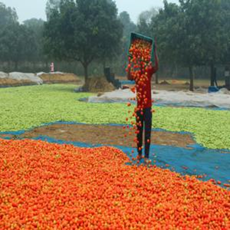
\includegraphics[width=\linewidth]{03-boundary/orangesea.png}
  \end{subfigure}
  \begin{subfigure}[b]{0.2\linewidth}
    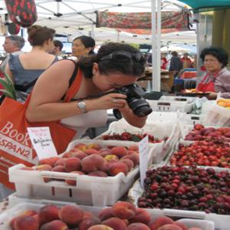
\includegraphics[width=\linewidth]{03-boundary/fruitmarket.png}
  \end{subfigure}
  \begin{subfigure}[b]{0.2\linewidth}
    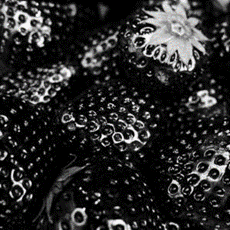
\includegraphics[width=\linewidth]{03-boundary/edits.png}
  \end{subfigure}
  \begin{subfigure}[b]{0.2\linewidth}
    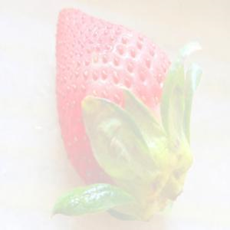
\includegraphics[width=\linewidth]{03-boundary/faded.png}
  \end{subfigure}
  \caption{Some boundary cases}
  \label{fig:img-boundary}
\end{figure}

\end{document}